% !TEX TS-program = xelatex
% !TEX encoding = UTF-8 Unicode
% !Mode:: "TeX:UTF-8"

\documentclass{resume}
\usepackage{zh_CN-Adobefonts_external} % Simplified Chinese Support using external fonts (./fonts/zh_CN-Adobe/)
% \usepackage{NotoSansSC_external}
% \usepackage{NotoSerifCJKsc_external}
% \usepackage{zh_CN-Adobefonts_internal} % Simplified Chinese Support using system fonts
\usepackage{linespacing_fix} % disable extra space before next section
\usepackage{cite}
\usepackage{graphicx} %导入graphics包
\usepackage{multirow}
\usepackage{tabu}
\usepackage{progressbar}
\begin{document}
\pagenumbering{gobble} % suppress displaying page number

\name{湛志强}
%\basicInfo{
%  \email{zhanzhiqiang09@126.com} \textperiodcentered\ 
%  \phone{(+86) 156-0060-2638} \textperiodcentered\ 
%  \faWechat{\ zhanzhiqiang09}
% % \linkedin[billryan8]{https://www.linkedin.com/in/billryan8}
% \includegraphics[width=0.12\textwidth]{/Users/zhanzq/Documents/2.jpg} %插入图片并设置宽度为页面的一半
%  }
  
\Large{
  \begin{tabu}{ c l r }
   \multirow{5}{1in}{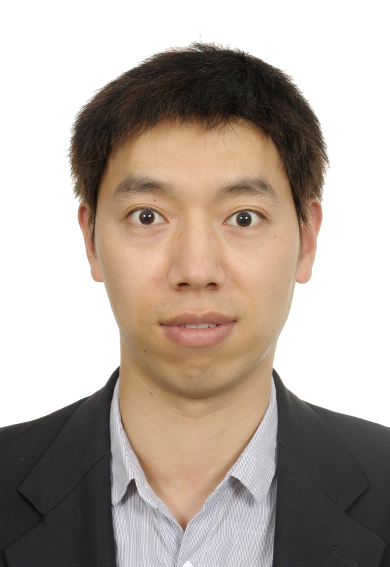
\includegraphics[width=0.88in, height=1.15in]{photo}} & \scshape{户籍：北京市朝阳区}  \\
   %& \scshape{Zhiqiang Zhan} & {C++~}\progressbar{0.8} \\
    & \scshape{出生年月：1988年7月} \\
    & \email{邮箱：zhanzhiqiang09@126.com} \\
    & \phone{电话: 156-0060-2638} \\
    & \scshape{求职意向：北方工业大学—信息学院—教学科研岗}
 %   & \linkedin[billryan8]{https://www.linkedin.com/in/billryan8}\\
 %   & \github[github.com/billryan]{https://github.com/billryan}
  \end{tabu}
}
 

\section{\faGraduationCap\  教育背景}
\datedsubsection{\textbf{中科院计算所} \ \ 北京}{2013 -- 2020}
\textit{博士}\ 计算机科学与技术
\datedsubsection{\textbf{吉林大学}\ \ 吉林, 长春}{2009 -- 2013}
\textit{学士}\ 计算机科学与技术

\section{\faUsers\ 工作经历}
\datedsubsection{\textbf{海尔优家} \ \ \ NLP算法专家} {2023.1 -- 至今}
\datedsubsection{\textbf{小鹏汽车} \ \ \ 资深算法工程师}{2021.9 -- 2023.1}
\datedsubsection{\textbf{联想研究院} \ \ 深度学习算法研究员}{2020.10 -- 2021.9}

\section{\faUsers\ 项目经历}
%\datedsubsection{\textbf{用户软件行为预测}}{2014年 -- 2015年}
%\role{Researcher}{个人项目，经理：葛付江}
%\begin{onehalfspacing}
%\emph{项目简介}：基于用户的历史数据，使用Seq2Seq深度学习模型预测用户的软件行为(总的软件数目为79个左右)。\\
%\emph{成果}：
%\begin{itemize}
%  \item top1的预测准确率达到41\%
%  \item top5的预测准确率达到67\%
%\end{itemize}
%\end{onehalfspacing}



\datedsubsection{\textbf{智能交互系统开发及优化}{\ (海尔优家)}}{2023年1月 -- 至今}

\role{\emph{Role:} 主要参与人员}{}
\begin{onehalfspacing}
\emph{项目简介}：以多种智能家电为入口，打造全屋智能环境。通过分布式唤醒，随时随地快速准确地理解用户指令，并及时做出响应，帮用户轻松控制各种家电设备，提供更舒适的生活方式。
\\
\emph{成果}：
\begin{itemize}
  \item 实现了冰、洗、空等100多个家电领域的语音交互及互联互通
  \item 构建了完善的模型预测 + 模板检索的意图理解及槽位提取方案，NLU准确率达到99+\%
  \item 语句改写、上下文继承、多意图理解、多模态拒识等显著提升了用户的交互成功率
\end{itemize}
\end{onehalfspacing}


\datedsubsection{\textbf{LLM研究与模型训练}{\ (海尔优家)}}{2023年1月 -- 至今}

\role{\emph{Role:} 主要参与人员}{}
\begin{onehalfspacing}
\emph{项目简介}：研究基于Transformer架构的类ChatGPT相关技术，探索LLM在智慧家电领域的应用，使之赋能海尔智慧家庭解决方案，达到降本增效的目的。同时，研究LLM的训练方法和优化技术，为智能家电领域的类ChatGPT模型的训练及应用进行技术积淀。
\\
\emph{成果}：
\begin{itemize}
  \item 对GPT系列的相关模型及核心技术进行了深入研究
  \item 对大模型的训练、微调及推理优化方法进行了较全面的研究学习，包括RLHF，ZeRO，FSDP，LoRA等优化技术，SparseAttention，1bit-Adam，Offload等训练技术和方法
  \item 在智能家电领域详细对比评测了多种主流的模型，如ChatGPT, ChatGLM, Xinghuo等
  \item 微调了开源的ChatGLM模型，并使用fastLLM进行量化部署，用于闲聊服务
  \item 主要参与并设计了海尔优家的HomeGPT架构，并提交了相关的专利
\end{itemize}
\end{onehalfspacing}

%\datedsubsection{\textbf{业务功能优化}{\ (海尔优家)}}{2023年1月 -- 至今}
%\role{\emph{Role:} 主要参与人员}{}
%\begin{onehalfspacing}
%\emph{项目简介}：对各业务功能进行持续优化，不断提升模型的NLU能力，提升交互成功率，改善用户体验。
%\\
%\emph{成果}：
%\begin{itemize}
%  \item 使用LLM进行数据的泛化及标注，节省人工标注成本80\%
%  \item 优化多个领域的NLU模型，准确率大大提高（70-80\% ==> 95+\%）
%\end{itemize}
%\end{onehalfspacing}

\datedsubsection{\textbf{XP智能座仓新架构}{\ (北京小鹏汽车智能语音部)}}{2022年 -- 2023年1月}
\role{\emph{Role:} 主要参与人员}{}
\begin{onehalfspacing}
\emph{项目简介}：基于RASA和Amazon Conversation架构，设计并实现新一代的\textbf{端到端}的\textbf{数据驱动}的XP智能座仓架构，达到降本增效的目的。整个架构由{\it Fusion Console}，{\it NLU}, {\it Action Server}, {\it Tracker}等多个组件构成。主要参与并负责{\it NLG Server}的设计及实现。
\\
\emph{成果}：
\begin{itemize}
  \item 通过组件设计，取代了TPL方案，提高了判断逻辑的可解释性和组件的可复用性，降低了开发和维护成本
  \item 实现了TPL逻辑和NLG的解耦，提高了NLG的运营效率
\end{itemize}
\end{onehalfspacing}

\datedsubsection{\textbf{多人全双工对话}{\ (北京小鹏汽车智能语音部)}}{2022年 -- 2023年1月}
\role{\emph{Role:} 主要参与人员}{}
\begin{onehalfspacing}
\emph{项目简介}：设计并实现全场景语音2.0，友好地支持多人同时与小P进行语音交互。主要参与了回复管理模块，负责设计并实现音区的权限管理、音频通道资源的冲突及协调、抢占退化策略、回复融合等功能。
\\
\emph{成果}：
\begin{itemize}
  \item 设计并实现了改造现有TPL的方案，提高了TPL的可扩展性
  \item 开发了TPL校验工具，大大提升了语音交互功能的开发效率，降低了维护成本
  \item 实现了判断逻辑与回复话术的解耦，提高了回复话术的运营效率 
  \item 实现了多功能的回复管理模块，有力支持了小P多人全双工对话的能力
\end{itemize}
\end{onehalfspacing}


\datedsubsection{\textbf{多人点餐}{\ (北京小鹏汽车智能语音部)}}{2021年 -- 2022年}
\role{\emph{Role:} 主要参与人员}{}
\begin{onehalfspacing}
\emph{项目简介}：探索智能汽车作为新一代个人空间的应用场景，实现多人同时参与讨论的点餐方案。主要参与并负责整个pipeline的设计并实现，其中包括NER，ABSA，逻辑推理（实体归一化、指代消解等）、主动引导策略等模块。
\\
\emph{成果}：
\begin{itemize}
  \item 基于GlobalPointer模型，结合数据增强方法，实现了NER模型在测试集上F1 ≥ 96\%
  \item 基于ABSA模型(Bert-SPC)，结合数据增强方法，实现了ABSA模型在测试集上F1 ≥ 95\%
  \item 基于上下文信息，实现了前指类型的指代消解~100\%的准确率
  \item 基于edit-distance算法和预置词表，实现了实体归一化~100\%的准确率
  \item 较好地完成了demo的交付
\end{itemize}
\end{onehalfspacing}

\datedsubsection{\textbf{表格数据生成文本}{\ (联想研究院)}}{2020年 -- 2021年}
\role{\emph{Role:} 主要负责人}{}
\begin{onehalfspacing}
\emph{项目简介}：使用GAN模型根据表格数据生成对应的文本描述，同时提升模型生成文本的流畅度和忠诚度。\\
\emph{成果}：
\begin{itemize}
  \item 使用GAN模型避免了强化学习中的reward设计
  \item 同时解决了现有模型生成文本的流畅度和忠诚度问题
  \item 所提模型在多个评价指标(BLEU-4, ROUGE-4, PARENT)上优于baseline
\end{itemize}
\end{onehalfspacing}

\datedsubsection{\textbf{对话生成}{\ (联想研究院)}}{2020年 -- 2021年}
\role{\emph{Role:} 主要负责人}{}
\begin{onehalfspacing}
\emph{项目简介}：通过分析对比主流的对话生成模型，我们总结了它们共有的问题：生成的应答多样性低、信息量少。经过数据分析，我们发现了可能的原因——语言学中的长尾效应。据此假设，我们提出了三种基于频率的数据正则化方法来解决长尾效应，从而提升对话生成模型的性能。
\\
\emph{成果}：
\begin{itemize}
  \item 三种数据正则化方法便捷高效，通用性强
  \item 能够有效提升模型生成应答的多样性和信息量
  \item 探索了一种改善对话生成模型的新思路
\end{itemize}
\end{onehalfspacing}


\datedsubsection{\textbf{GEC}{\ (联想研究院)}}{2020年 -- 2020年}
\role{\emph{Role:} 主要负责人}{}
\begin{onehalfspacing}
\emph{工作简介}：基于GECToR模型，我们采用数据增强、模型级联和模型融合方法，提升了模型在BEA-2019任务上的性能表现。\\
\emph{成果}：
\begin{itemize}
  \item 刷新了BEA-2019 Restricted Track上的纪录，取得了F0.5=\textbf{75.39\%}
\end{itemize}
\end{onehalfspacing}

\section{\faUsers\ 实习/研究经历}
\datedsubsection{\textbf{英语口语评分引擎}{\ (联想研究院)}}{2019年 -- 2020年}
\role{\emph{Role:} 主要负责人}{}
\begin{onehalfspacing}
\emph{项目简介}：利用预训练的语音转文本模型OpenSeq2Seq解析语音数据，使用神经网络模型对抽取的特征进行训练以拟合人工评分，对测试数据进行模型评分。\\
\emph{成果}：
\begin{itemize}
  \item 神经网络评分模型结构简单，速度快
  \item 模型评分与人工评分有高度的一致性，pearson相关系数达到0.91
\end{itemize}
\end{onehalfspacing}

\datedsubsection{\textbf{对话生成评价}{\ (联想研究院)}}{2016年 -- 2020年}
\role{\emph{Role:} 主要负责人}{}
\begin{onehalfspacing}
\emph{项目简介}：针对通用领域的对话生成系统，提出了一个全面的(语义连贯性、语法正确性和模型整体表达能力)评价指标SSA。并设计、实现了语义评价模型和语法评价模型。\\
\emph{成果}：
\begin{itemize}
  \item SSA与人工评价的相关性远远高于传统的评价指标(包括BLEU, METEOR, ROUGE)
  \item 在数据集层面上，相关性系数提高了0.29-0.35
  \item 在模型层面上，相关性系数提高了0.23-0.30
  \item 可以明确从语义和语法角度评价生成的句子
\end{itemize}
\end{onehalfspacing}

\datedsubsection{\textbf{文本分类}{\ (联想研究院)}}{2017年 -- 2019年}
\role{\emph{Role:} 主要负责人}{}
\begin{onehalfspacing}
\emph{项目简介}：融合文本的语义信息和结构信息，构建文本的表示模型，并进行文本分类。\\
\emph{成果}：
\begin{itemize}
  \item 融合了语义和结构信息，并使用self-attention进行权重计算
  \item 在3个公开数据集上达到了当时最高的准确率(不使用句法解析树)
\end{itemize}
\end{onehalfspacing}

\datedsubsection{\textbf{融合知识的对话生成}{\ (联想研究院)}} {2015年 -- 2016年}
\role{\emph{Role:} 主要负责人}{}
\begin{onehalfspacing}
\emph{项目简介}：从百度百科抽取三元组知识，结合Seq2Seq模型，构建了融合知识的对话生成系统。\\
\emph{成果}：
\begin{itemize}
  \item 大大降低了模型复杂度，提高了模型训练速度
  \item 可根据不能输入的风格，生成不同的输出响应
  \item 在5个语义类别的测试集上的语义准确率达到了98\%以上
\end{itemize}
\end{onehalfspacing}


%\datedsubsection{\textbf{量化模型的鲁棒性}{\ (联想研究院)}}{2021年 -- 至今}
%\role{Researcher}{经理：张杨，与李睿易、龚江涛合作研究}
%\begin{onehalfspacing}
%\emph{项目简介}：现有的神经网络模型容易受到对抗样本的攻击，为了评估模型的抗攻击能力(即模型的鲁棒性)，我们提出了一种量化指标TCFV。我们使用TCFV在两个数据集上进行了3种主流分类模型对三种攻击方法的实验，分析了模型特定层的鲁棒性、攻击方法的特性及攻击方法对模型的具体影响等，验证了量化指标TCFV的有效性。
%\\
%\emph{成果}：
%\begin{itemize}
%  \item 提出了一种模型鲁棒性的量化指标
%  \item 分析了模型复杂度和鲁棒性的相关性及不同攻击方法的特性
%  \item 分析了模型特定层的鲁棒性，为模型的改善提供建议
%\end{itemize}
%\end{onehalfspacing}


\section{发表论文}
\datedsubsection{1. \textbf{Adaptive Learning of Local Semantic and Global Structure Representations for Text Classification, Coling, CCF B会议}}{April, 2018}

\datedsubsection{2. \textbf{SSA: A More Humanized Automatic Evaluation Method for Open Dialogue Generation, IJCNN, CCF C会议}}{July, 2019}

\datedsubsection{3. \textbf{MIDS: End-to-End Personalized Response Generation in Untrimmed Multi-Role Dialogue, IJCNN, CCF C会议}}{July, 2019}

\datedsubsection{4. \textbf{End-to-End Personalized Humorous Response Generation in Untrimmed Multi-Role Dialogue System, IEEE Access, SCI 二区}}{Auguest, 2019}

\datedsubsection{5. \textbf{Introspection Unit in Memory Network: Learning to Generalize Inference in OOV Scenarios, NeuroComputing, SCI二区}}{October, 2019}

\datedsubsection{6. \textbf{Knowledge Attention Sandwich Neural Network for Text Classification, NeuroComputing, SCI 二区}}{April, 2020}

\datedsubsection{7. \textbf{Generative adversarial network for Table-to-Text generation, NeuroComputing, SCI 二区}}{April, 2021}

\datedsubsection{8. \textbf{Grabbing the Long Tail: A Data Normalization Method for Diverse and Informative Dialogue Generation, NeuroComputing, SCI二区}}{July, 2021}

%\datedsubsection{9. \textbf{Interpreting Robustness of Deep Neural Networks With RepresentationalSimilarity Analysis}}{AAAI2022在投}

\section{申请专利}
\datedsubsection{1. \textbf{一种口语测评方法、设备及计算机可读存储介质 [发明]}}{申请号：CN202010127185.8}{公开日：2020.07.10}

\datedsubsection{2. \textbf{一种文本评分方法、电子设备和计算机可读存储介质 [发明]}}{申请号：CN202110129208.3}{公开日：2021.05.11}

\datedsubsection{3. \textbf{试题生成方法及装置 [发明]}}{申请号：CN202110185141.5}{公开日：2021.05.14}

\datedsubsection{4. \textbf{一种信息处理方法、设备及存储介质 [发明]}}{申请号：CN202110896685.2}{公开日：2021.12.07}

\datedsubsection{5. \textbf{数据处理方法、装置及电子设备 [发明]}}{申请号：CN202111045487.1}{公开日：2021.12.07}

\datedsubsection{6. \textbf{一种信息处理方法、装置和电子设备 [发明]}}{申请号：CN202111120210.0}{公开日：2021.12.28}

\datedsubsection{7. \textbf{语音交互方法、服务器及计算机可读存储介质 [发明]}}{申请号：CN202211551227.6}{公开日：2023.01.06}


\section{\faHeartO\ 获奖情况}
\datedline{国家励志奖学金}{2010-2011}
\datedline{国家励志奖学金}{2011-2012}
\datedline{国家励志奖学金}{2012-2013}
\datedline{校三好学生}{2015-2016}
\section{\faCogs\ IT 技能}
% increase linespacing [parsep=0.5ex]
\begin{itemize}[parsep=0.5ex]
  \item 编程语言：精通Python、C和C++，熟悉Java
  \item 平台：Linux
  \item 深度学习框架：精通tensorflow和pytorch，熟悉keras和theano
\end{itemize}

%\section{\faInfo\ 个人编程主页}
%% increase linespacing [parsep=0.5ex]
%\begin{itemize}[parsep=0.5ex]
%  \item leetcode: https://leetcode.com/zhanzq/
%    \item leetcode-cn: https://leetcode-cn.com/zhanzq/
%  \item lintcode: https://www.lintcode.com/user/zhanzq/
%\end{itemize}

%% Reference
%\newpage
%\bibliographystyle{IEEETran}
%\bibliography{resume_zzq_zh}
\end{document}
